% Latex template: mahmoud.s.fahmy@students.kasralainy.edu.eg
% For more details: https://www.sharelatex.com/learn/Beamer

\documentclass{beamer}					  % Document class

\usepackage[portuguese]{babel}			  % Set language
\usepackage[utf8x]{inputenc}			  % Set encoding

\mode<presentation> {					  % Set options
  \usetheme{default}					    % Set theme
  \usecolortheme{default} 				% Set colors
  \usefonttheme{default}  				% Set font theme
  \setbeamertemplate{caption}[numbered]	% Set caption to be numbered
}

\setbeamertemplate{navigation symbols}{}
\setbeamertemplate{footline}[frame number]
\setbeamercovered{transparent}

% Uncomment this to have the outline at the beginning of each section highlighted.
%\AtBeginSection[]
%{
%  \begin{frame}{Outline}
%    \tableofcontents[currentsection]
%  \end{frame}
%}

\usepackage{graphicx}					% For including figures
\usepackage{booktabs}					% For table rules
\usepackage{hyperref}					% For cross-referencing
\usepackage{caption}                    % Allows more control over captions in figs and tables

\title{Revisão de Atividades da FAC}	% Presentation title
%\author{Author One}					% Presentation author
\institute{LNLS.DAC.FAC}				% Author affiliation
\date{2024-01-26 -- 2024-02-16}			% Today's date	


\begin{document}



\begin{frame}
  \titlepage
  \href{https://github.com/lnls-fac/doc-review-dac-fac}{\beamergotobutton{Link para o repo github desta apresentação: https://github.com/lnls-fac/doc-review-dac-fac}}
  \href{https://www.overleaf.com/read/sbdjxtzfchrm}{\beamergotobutton{Link para o projeto overleaf destas notas}}
\end{frame}

\begin{frame}{Outline}
  \tableofcontents
\end{frame}




\section{Instabilidades Transversais}

\begin{frame}{Instabilidades Transversais}
    \scriptsize{\begin{itemize}
            \item Estudo de máquina 29/01, BbB
    \end{itemize}}
    \begin{figure}[H]
        	\centering
            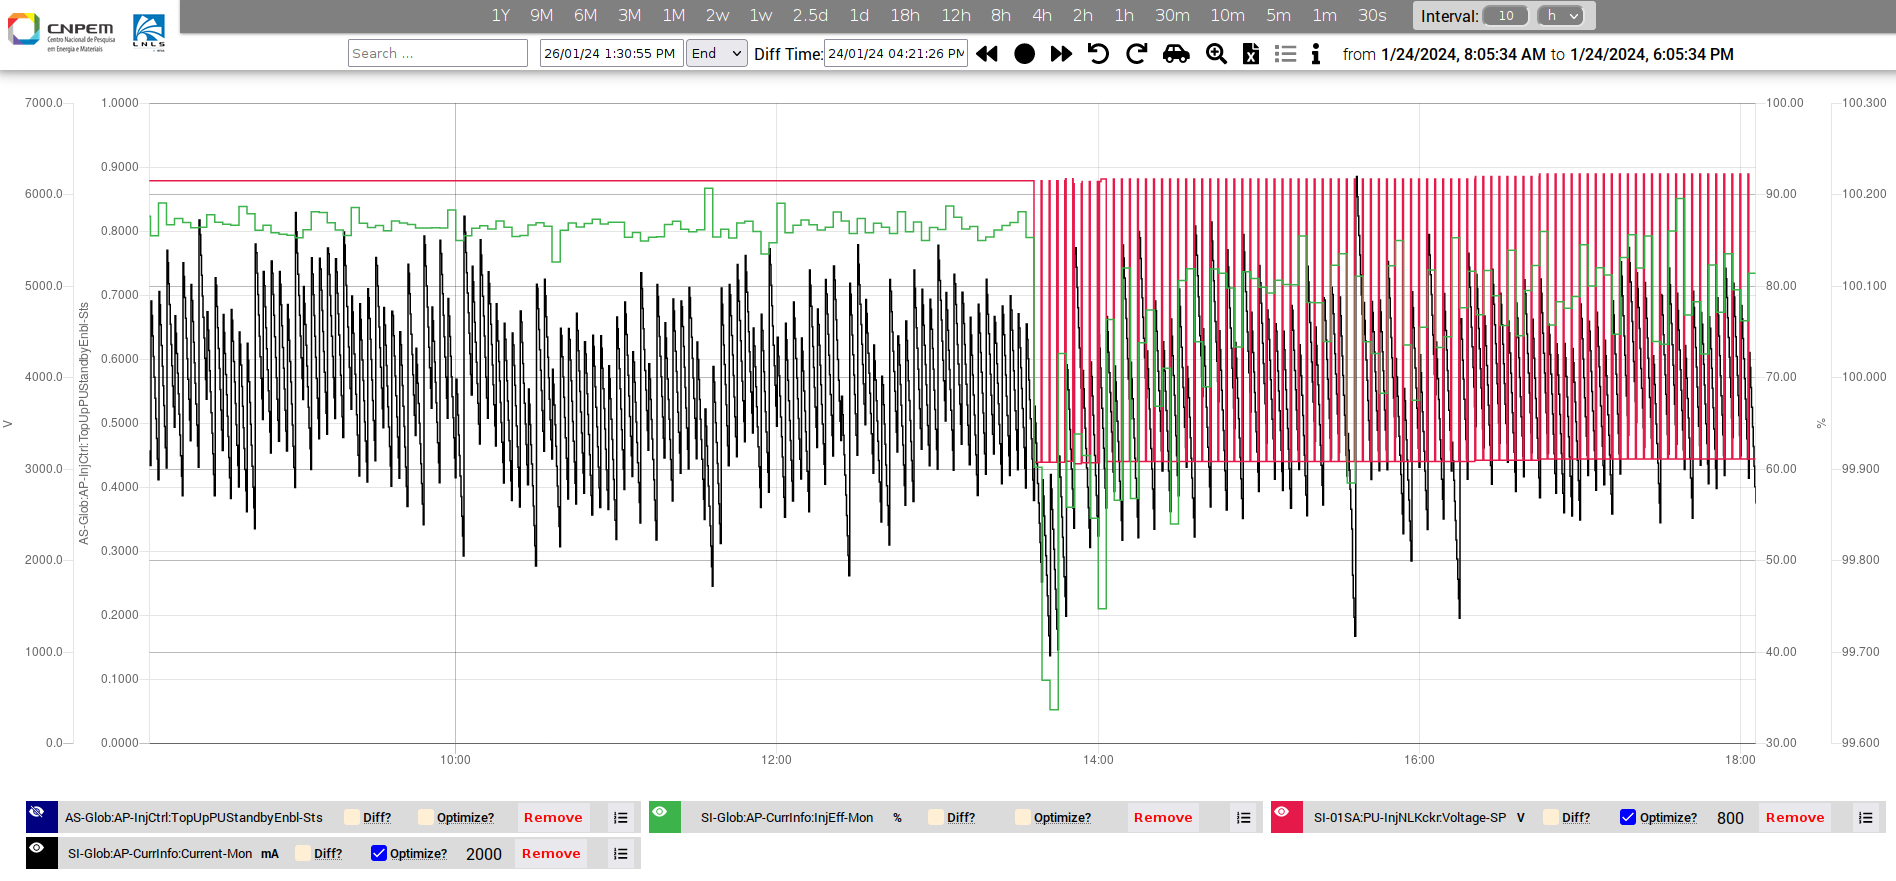
\includegraphics[width=0.8\textwidth]{2024-02-16/figures/pu-standby.png}
            \label{fig:pu-standby}
    \end{figure} 
\end{frame}



\section{NLK}

\begin{frame}{NLK - kick horizontal}
    \scriptsize{\begin{itemize}
    		\item Feixe localizado
            \item Varredura do pulso NLK com relação ao feixe
    \end{itemize}}
    \begin{figure}[H]
        	\centering
            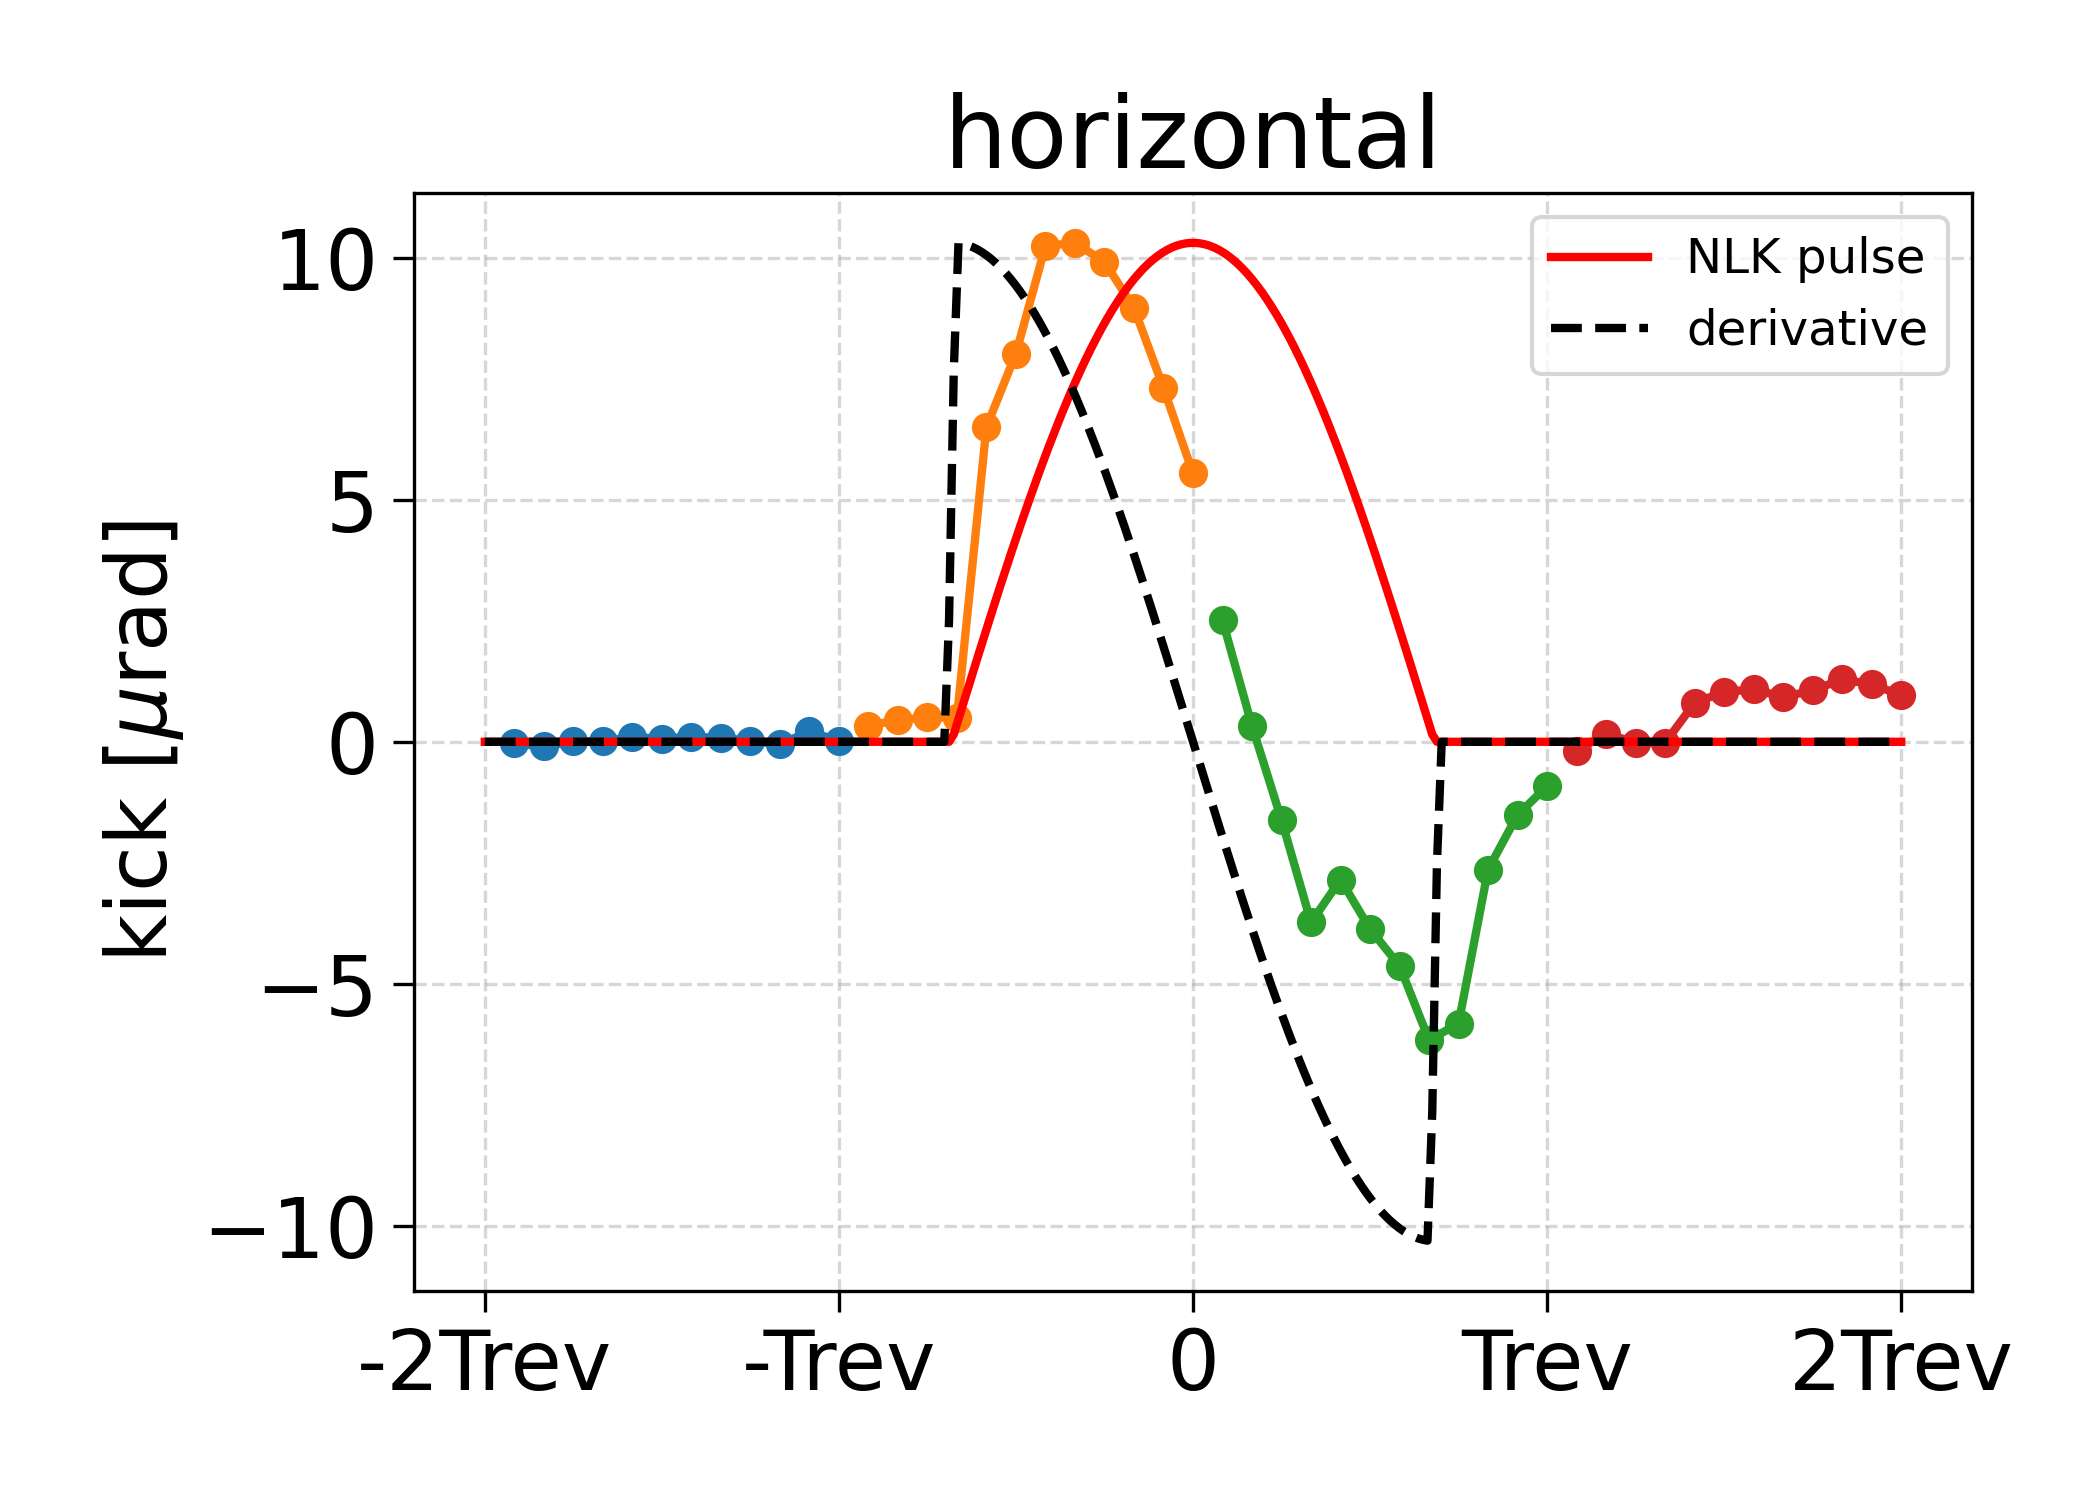
\includegraphics[width=0.8\textwidth]{2024-02-16/figures/nlk_horizontal_kick_profile.png}
            \label{fig:nlk-h-kick-profile}
    \end{figure} 
\end{frame}

\begin{frame}{NLK - kick vertical}
    \scriptsize{\begin{itemize}
    		\item Feixe localizado
            \item Varredura do pulso NLK com relação ao feixe
    \end{itemize}}
    \begin{figure}[H]
        	\centering
            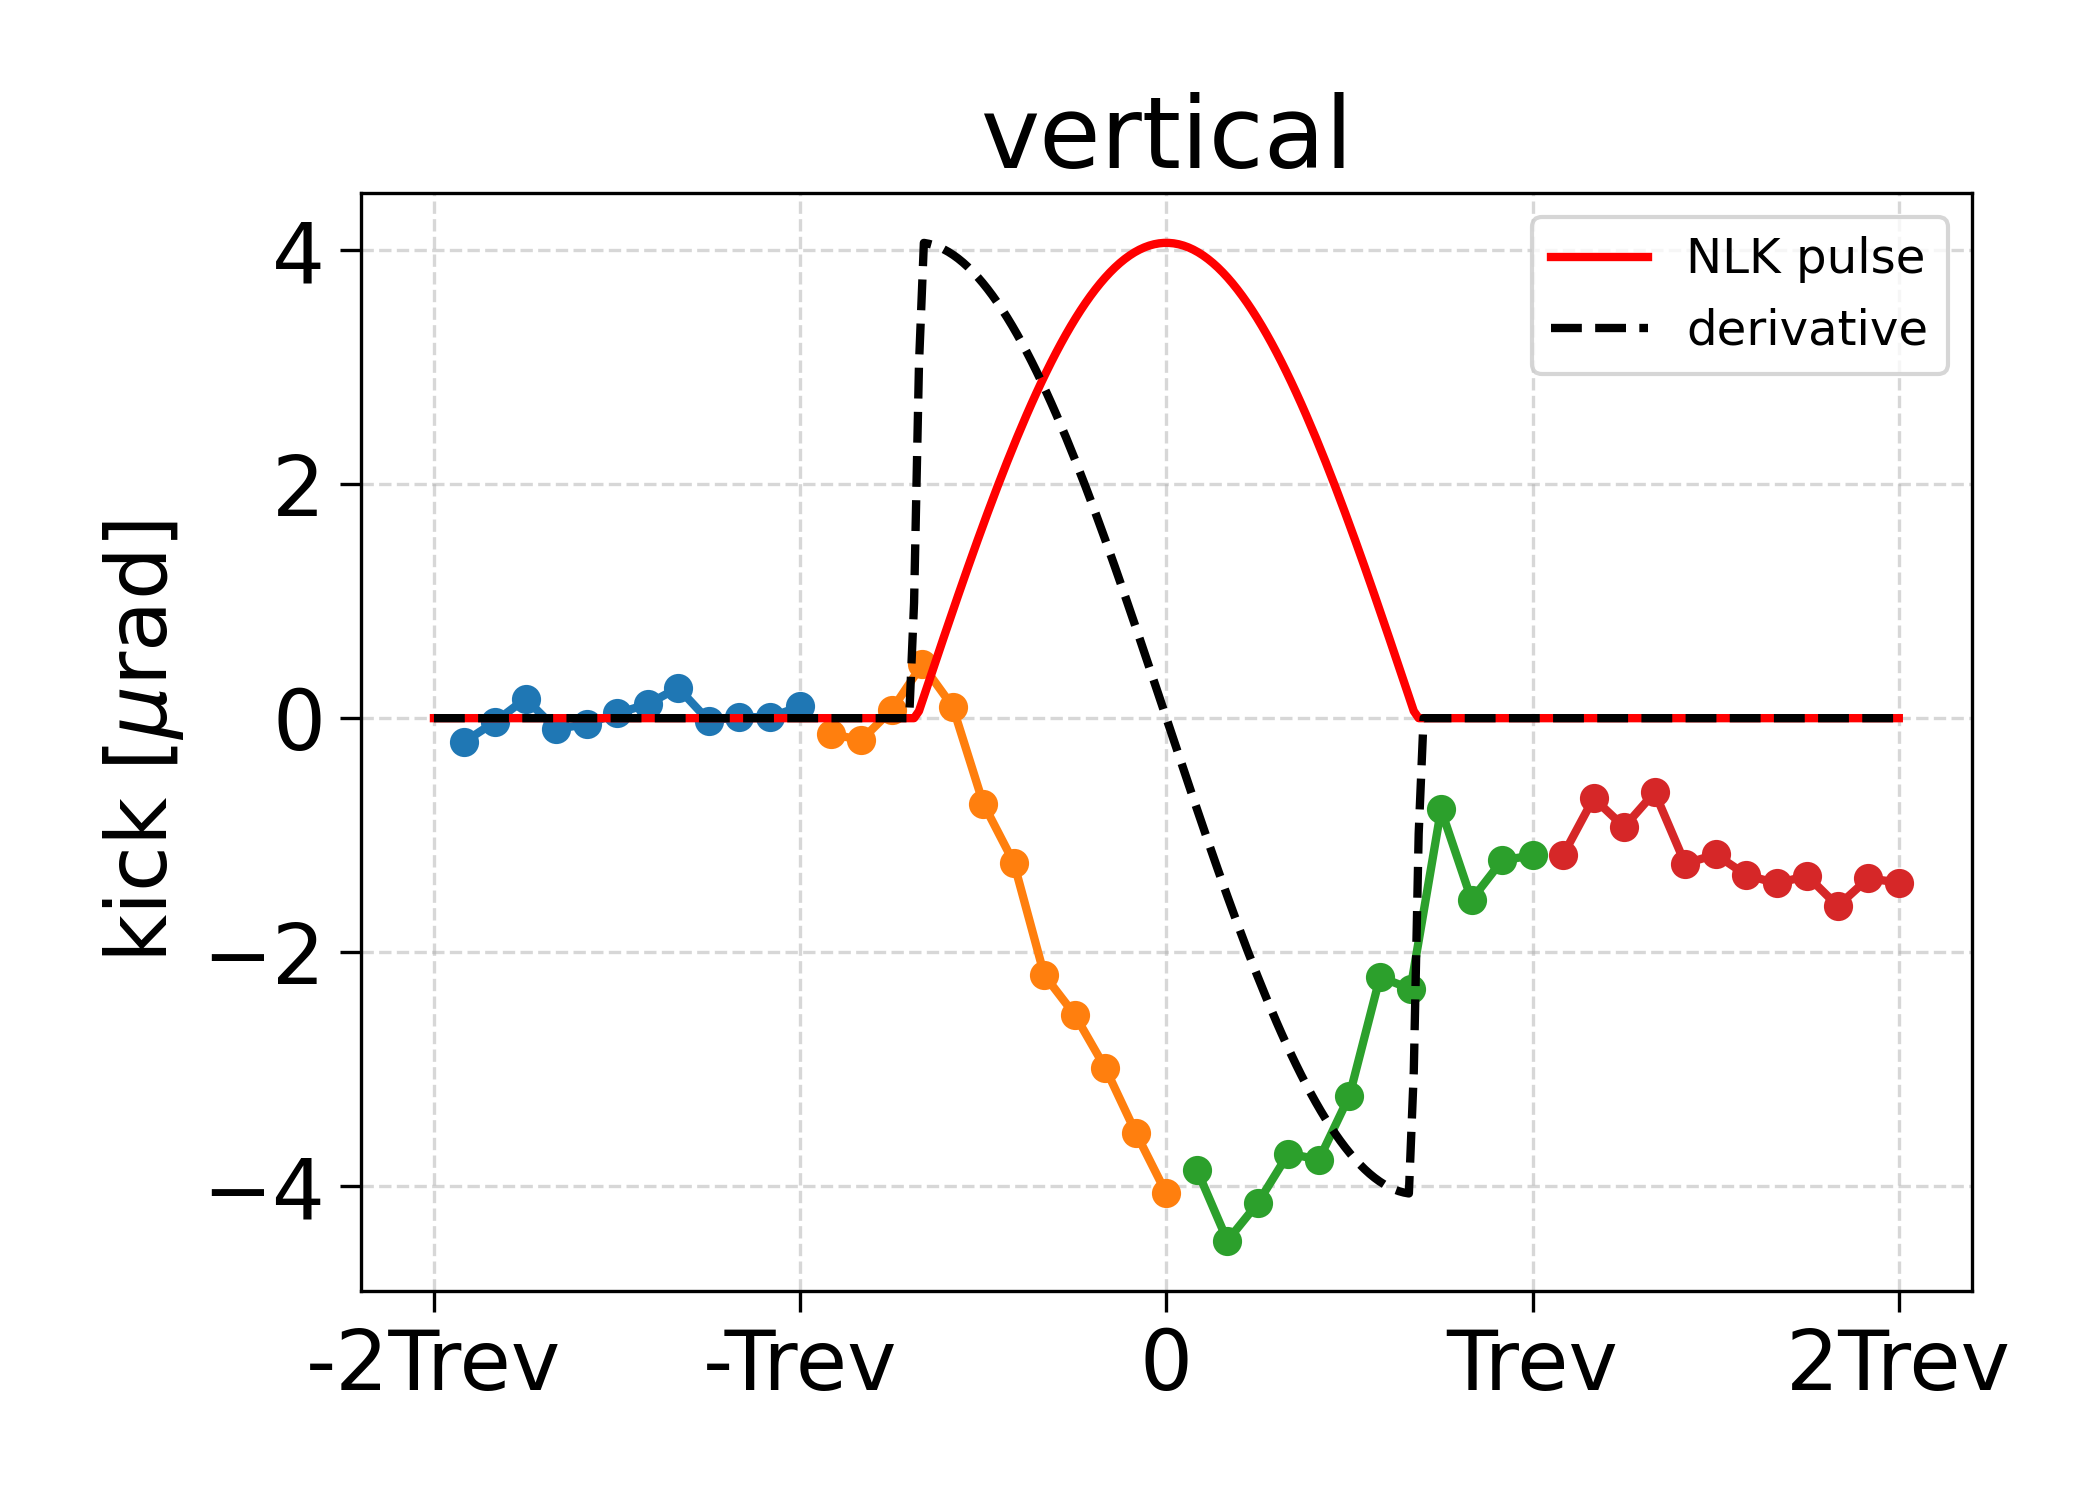
\includegraphics[width=0.8\textwidth]{2024-02-16/figures/nlk_vertical_kick_profile.png}
            \label{fig:nlk-v-kick-profile}
    \end{figure} 
\end{frame}

\begin{frame}{Comparativo da perturbação no centroide (BPM-01M2)}
    \begin{figure}[H]
        	\centering
            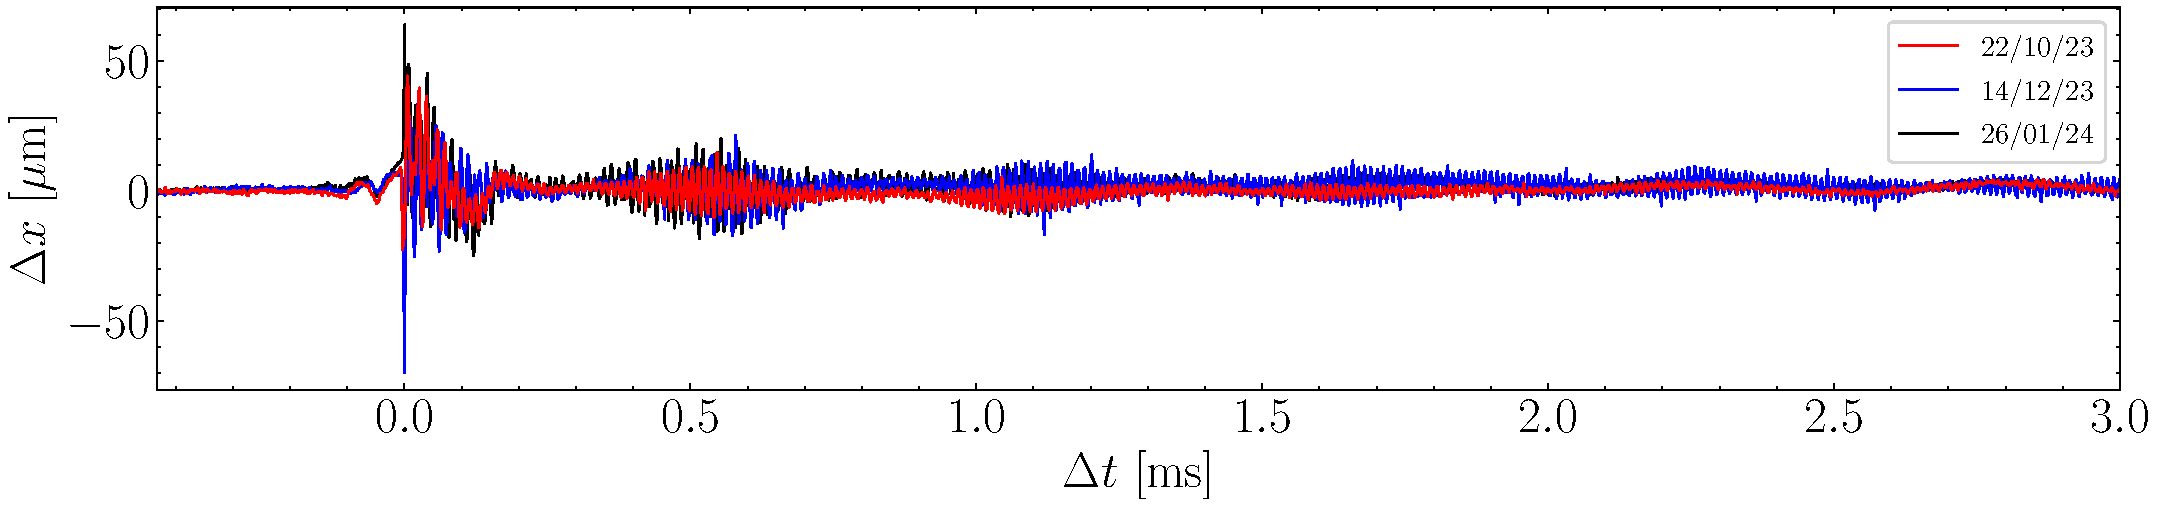
\includegraphics[width=1.0\textwidth]{2024-02-16/figures/injection_perturbation_compare_x_2024.pdf}
            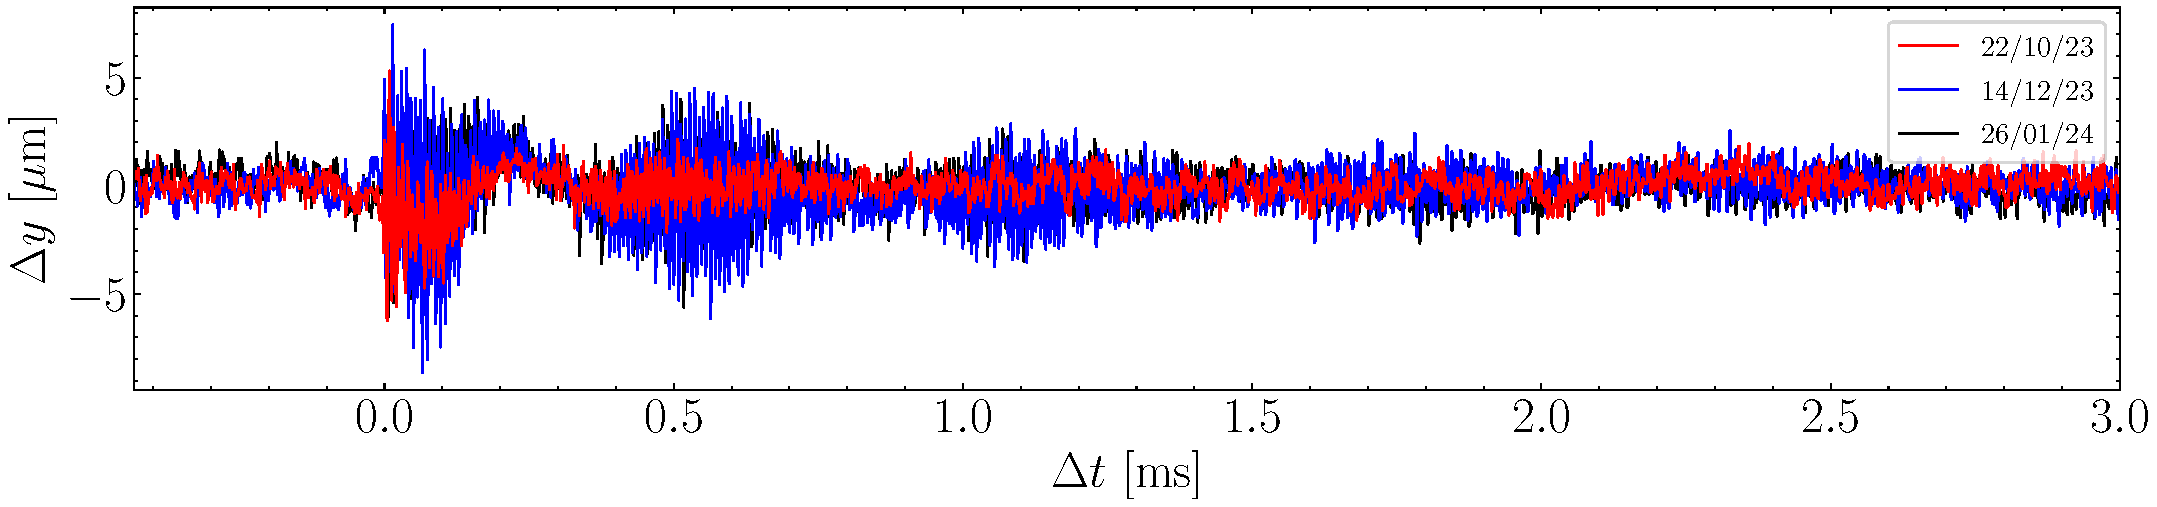
\includegraphics[width=1.0\textwidth]{2024-02-16/figures/injection_perturbation_compare_y_2024.pdf}
    \end{figure} 
\end{frame}



\section{Ótica do Booster}

\begin{frame}{Ótica do Booster}
    \begin{itemize}
        \item Movimentação do DELTA provoca a) distorções de órbita, b) mudança de acomplamento, c) distorção das funções beta, d) mudança da abertura dinâmica, tempo de vida, tc.
    \end{itemize}
    \begin{figure}[H]
    		\centering
            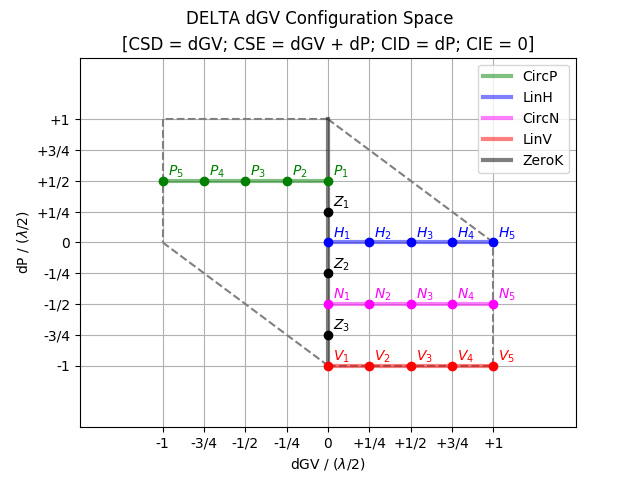
\includegraphics[width=.8\textwidth]{2024-02-16/figures/id-delta-dgv-config-space.png}
            \caption{Espaço de configuração do DELTA}
            \label{fig:delta-config-space}
    \end{figure}
\end{frame}



\section{References}



\end{document}
